\pagestyle{empty}
\chapter*{\centering \large DAFTAR RIWAYAT HIDUP}
\thispagestyle{empty}

\begin{wrapfigure}{l}{4cm}
	\vspace{-25pt}
	\begin{center}
		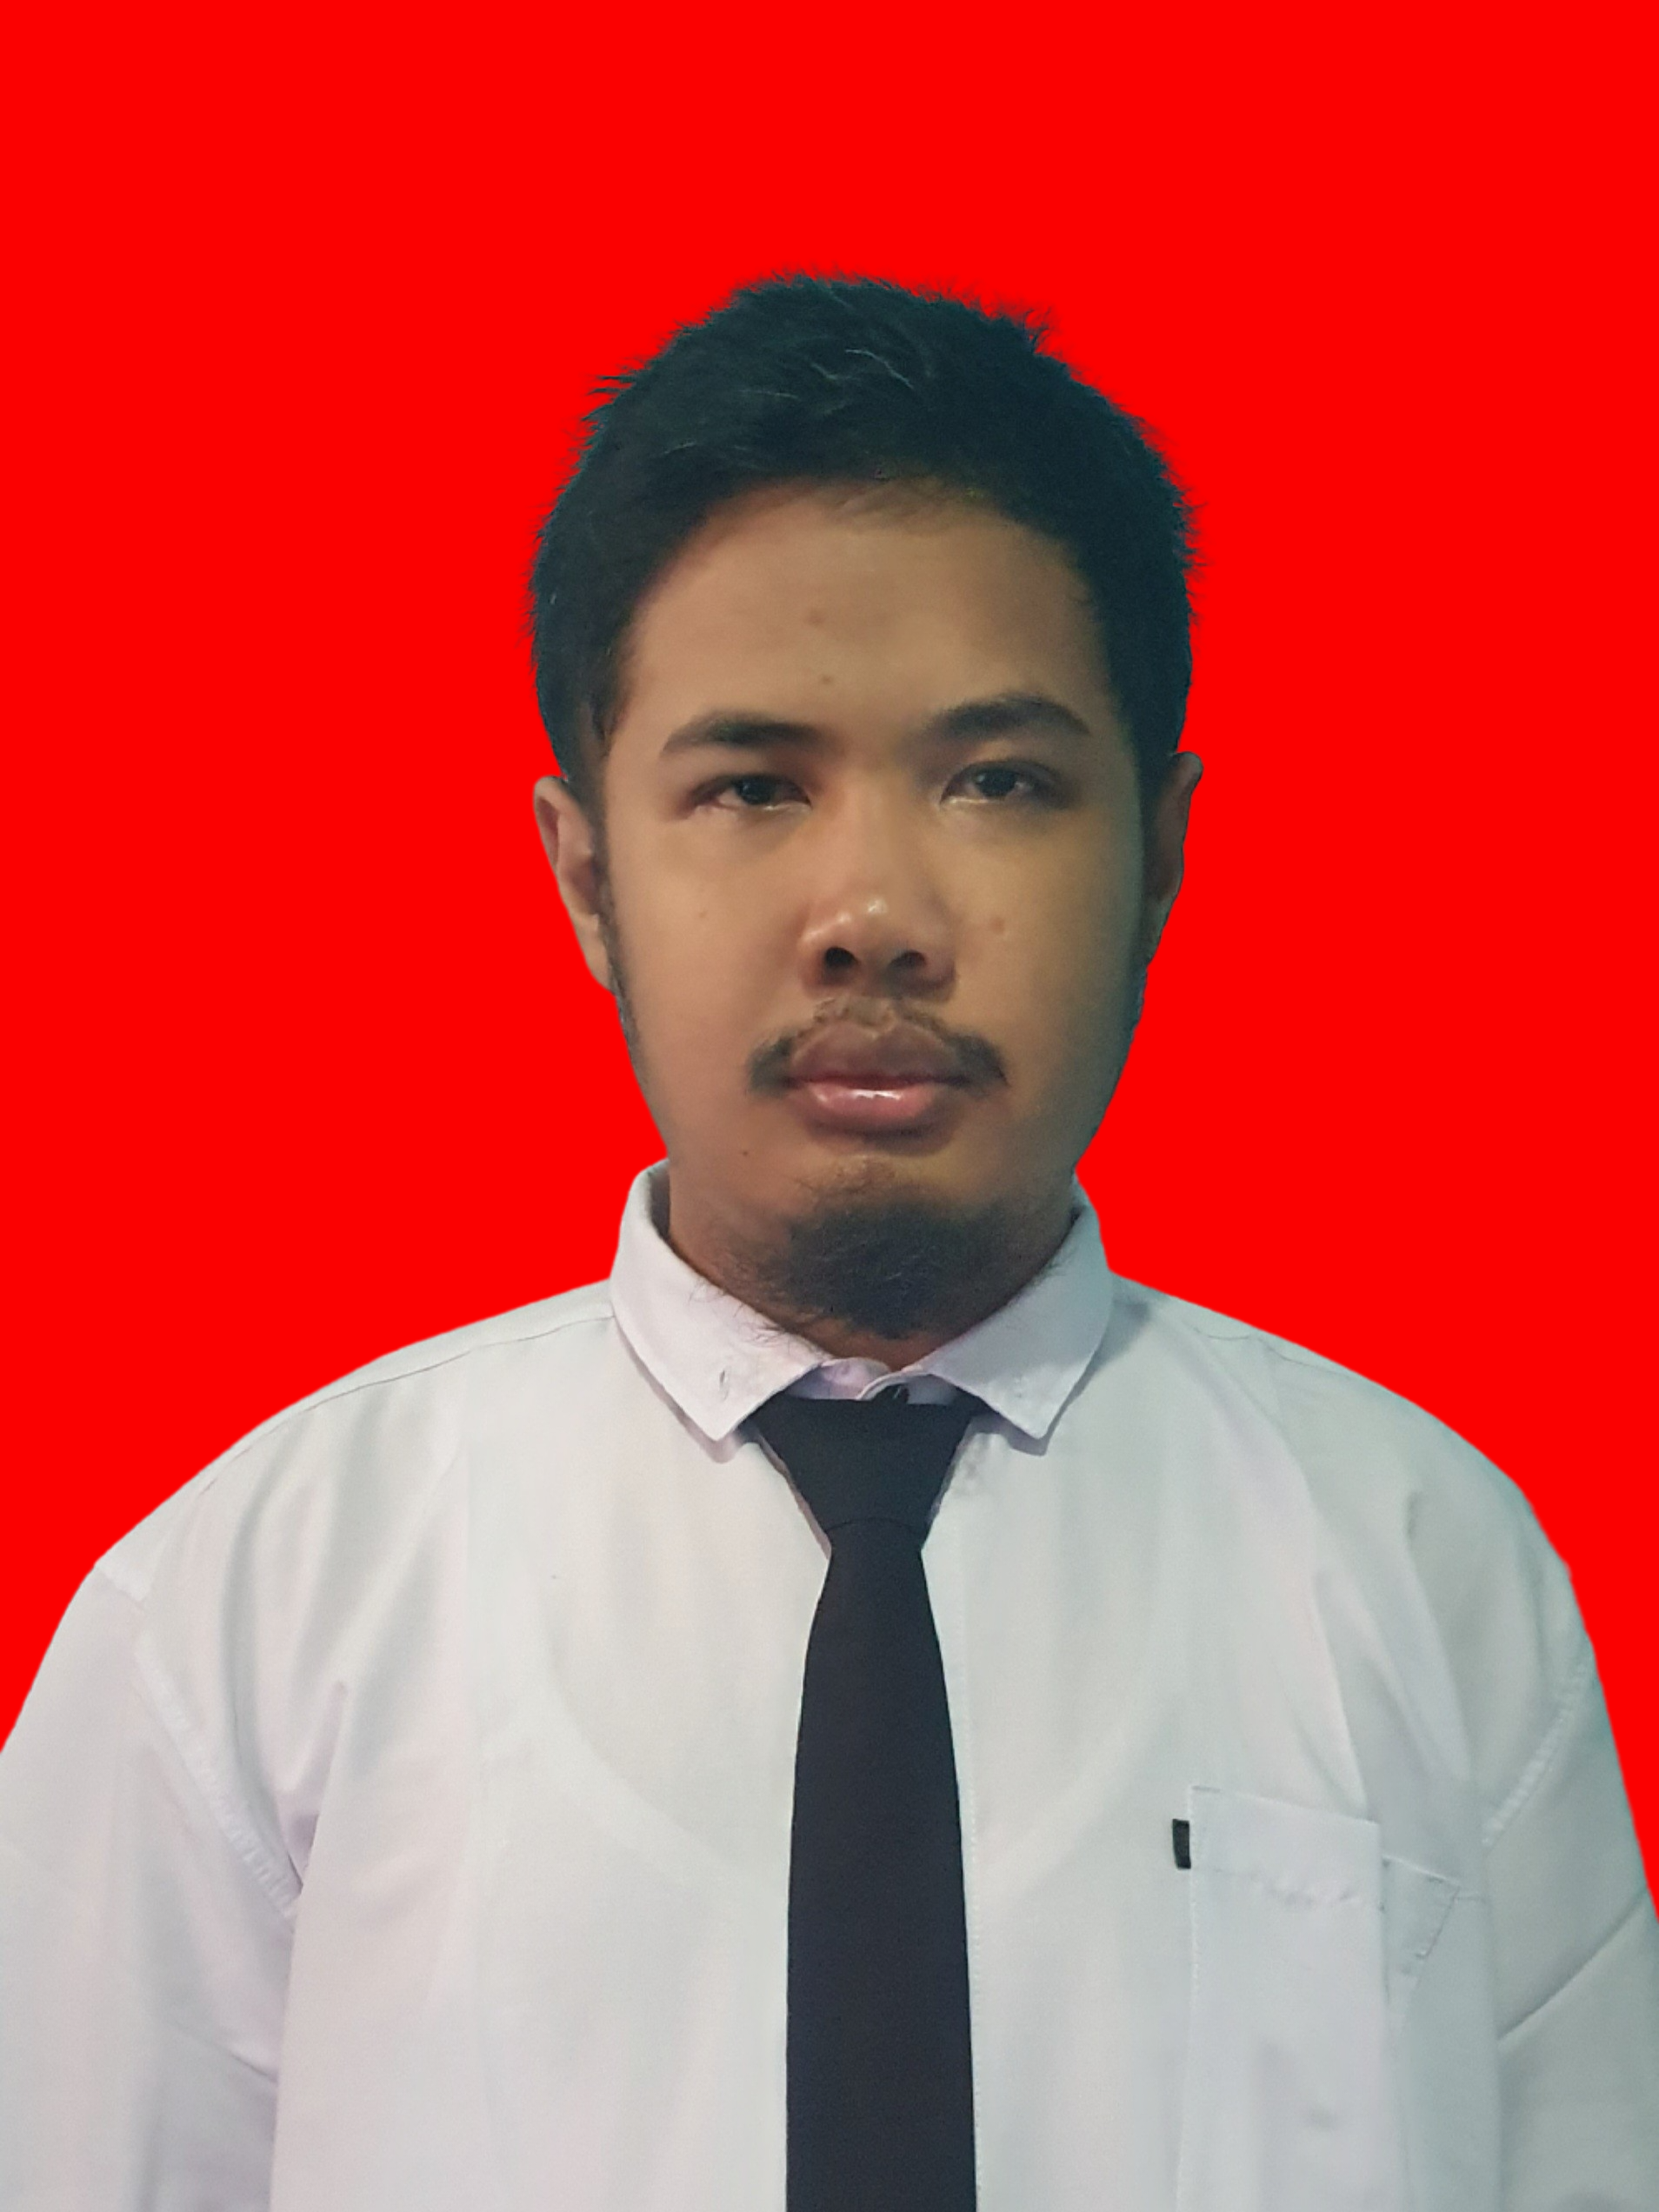
\includegraphics[width=0.27\textwidth]{gambar/pas-foto}
	\end{center}
	\vspace{-80pt}
\end{wrapfigure}

\noindent \textbf{MUHAMMAD INSAN KHAMIL.}  Lahir di Boyolali, 21 Febuari 1998.  Anak pertama dari pasangan Bapak Sriyono dan Ibu Inong Martini. Saat ini beralamatkan di Jl. Mawar 2 no. 5C RT 08 RW 13 kel. Bintaro kec. Pesanggrahan, Kota Jakarta Selatan.

\vspace{0.5cm}
\noindent
\begin{center}
	\begin{flushright}
		\begin{tabular}{lcl}
			No. Ponsel	& :&  081293402756 \\
			Email	& :& khami\_insan0@yahoo.com
		\end{tabular}
	\end{flushright}
\end{center}
\vspace{0.5cm}

\noindent \textbf{Riwayat Pendidikan} : Penulis mengawali pendidikan di MIN 15 Bintaro pada tahun 2004 - 2010. Setelah itu, penulis melanjutkan studi ke SMPN 178 Jakarta hingga tahun 2013. Kemudian melanjutkan ke SMAN 87 Jakarta hingga tahun 2016. Di Tahun 2016 penulis melanjutkan ke Universitas Negeri Jakarta (UNJ), Program Studi Ilmu Komputer, melalui jalur SBMPTN dengan beasiswa BIDIKMISI dan kemudian lulus di tahun 2023.

\noindent \textbf{Riwayat Organisasi} : Selama di bangku perkuliahan, penulis tergabung dengan organisasi kemahasiswaan seperti, Masjid Ulul Albaab yang sekarang Lembaga Dakwah Ulul Albab sebagai staff Huda periode 2017 dan 2018. Penulis juga berpartisipasi dalam organisasi Badan Eksekutif Mahasiswa di Program Studi Ilmu Komputer periode 2018, dimana penulis tergabung sebagai kepala departemen rohani islam. Penulis juga kerap mengikuti kepanitiaan kegiatan yang diadakan oleh lembaga dakwah fakultas (MUA), dan komunitas atau \textit{underbow} lembaga (Default). 

\noindent \textbf{Tentang Skripsi} : Skripsi ini merupakan karya terbaik penulis yang diberikan untuk civitas akademika Universitas Negeri Jakarta. Besar harapan penulis agar skripsi ini dapat bermanfaat bagi semua yang membaca dan menggunakan hasil penelitian ini.